% Options for packages loaded elsewhere
\PassOptionsToPackage{unicode}{hyperref}
\PassOptionsToPackage{hyphens}{url}
%
\documentclass[
]{book}
\usepackage{lmodern}
\usepackage{amssymb,amsmath}
\usepackage{ifxetex,ifluatex}
\ifnum 0\ifxetex 1\fi\ifluatex 1\fi=0 % if pdftex
  \usepackage[T1]{fontenc}
  \usepackage[utf8]{inputenc}
  \usepackage{textcomp} % provide euro and other symbols
\else % if luatex or xetex
  \usepackage{unicode-math}
  \defaultfontfeatures{Scale=MatchLowercase}
  \defaultfontfeatures[\rmfamily]{Ligatures=TeX,Scale=1}
\fi
% Use upquote if available, for straight quotes in verbatim environments
\IfFileExists{upquote.sty}{\usepackage{upquote}}{}
\IfFileExists{microtype.sty}{% use microtype if available
  \usepackage[]{microtype}
  \UseMicrotypeSet[protrusion]{basicmath} % disable protrusion for tt fonts
}{}
\makeatletter
\@ifundefined{KOMAClassName}{% if non-KOMA class
  \IfFileExists{parskip.sty}{%
    \usepackage{parskip}
  }{% else
    \setlength{\parindent}{0pt}
    \setlength{\parskip}{6pt plus 2pt minus 1pt}}
}{% if KOMA class
  \KOMAoptions{parskip=half}}
\makeatother
\usepackage{xcolor}
\IfFileExists{xurl.sty}{\usepackage{xurl}}{} % add URL line breaks if available
\IfFileExists{bookmark.sty}{\usepackage{bookmark}}{\usepackage{hyperref}}
\hypersetup{
  pdftitle={Analyses for Tag-based Genetic Regulation for Genetic Programming},
  pdfauthor={Alexander Lalejini},
  hidelinks,
  pdfcreator={LaTeX via pandoc}}
\urlstyle{same} % disable monospaced font for URLs
\usepackage{color}
\usepackage{fancyvrb}
\newcommand{\VerbBar}{|}
\newcommand{\VERB}{\Verb[commandchars=\\\{\}]}
\DefineVerbatimEnvironment{Highlighting}{Verbatim}{commandchars=\\\{\}}
% Add ',fontsize=\small' for more characters per line
\usepackage{framed}
\definecolor{shadecolor}{RGB}{248,248,248}
\newenvironment{Shaded}{\begin{snugshade}}{\end{snugshade}}
\newcommand{\AlertTok}[1]{\textcolor[rgb]{0.94,0.16,0.16}{#1}}
\newcommand{\AnnotationTok}[1]{\textcolor[rgb]{0.56,0.35,0.01}{\textbf{\textit{#1}}}}
\newcommand{\AttributeTok}[1]{\textcolor[rgb]{0.77,0.63,0.00}{#1}}
\newcommand{\BaseNTok}[1]{\textcolor[rgb]{0.00,0.00,0.81}{#1}}
\newcommand{\BuiltInTok}[1]{#1}
\newcommand{\CharTok}[1]{\textcolor[rgb]{0.31,0.60,0.02}{#1}}
\newcommand{\CommentTok}[1]{\textcolor[rgb]{0.56,0.35,0.01}{\textit{#1}}}
\newcommand{\CommentVarTok}[1]{\textcolor[rgb]{0.56,0.35,0.01}{\textbf{\textit{#1}}}}
\newcommand{\ConstantTok}[1]{\textcolor[rgb]{0.00,0.00,0.00}{#1}}
\newcommand{\ControlFlowTok}[1]{\textcolor[rgb]{0.13,0.29,0.53}{\textbf{#1}}}
\newcommand{\DataTypeTok}[1]{\textcolor[rgb]{0.13,0.29,0.53}{#1}}
\newcommand{\DecValTok}[1]{\textcolor[rgb]{0.00,0.00,0.81}{#1}}
\newcommand{\DocumentationTok}[1]{\textcolor[rgb]{0.56,0.35,0.01}{\textbf{\textit{#1}}}}
\newcommand{\ErrorTok}[1]{\textcolor[rgb]{0.64,0.00,0.00}{\textbf{#1}}}
\newcommand{\ExtensionTok}[1]{#1}
\newcommand{\FloatTok}[1]{\textcolor[rgb]{0.00,0.00,0.81}{#1}}
\newcommand{\FunctionTok}[1]{\textcolor[rgb]{0.00,0.00,0.00}{#1}}
\newcommand{\ImportTok}[1]{#1}
\newcommand{\InformationTok}[1]{\textcolor[rgb]{0.56,0.35,0.01}{\textbf{\textit{#1}}}}
\newcommand{\KeywordTok}[1]{\textcolor[rgb]{0.13,0.29,0.53}{\textbf{#1}}}
\newcommand{\NormalTok}[1]{#1}
\newcommand{\OperatorTok}[1]{\textcolor[rgb]{0.81,0.36,0.00}{\textbf{#1}}}
\newcommand{\OtherTok}[1]{\textcolor[rgb]{0.56,0.35,0.01}{#1}}
\newcommand{\PreprocessorTok}[1]{\textcolor[rgb]{0.56,0.35,0.01}{\textit{#1}}}
\newcommand{\RegionMarkerTok}[1]{#1}
\newcommand{\SpecialCharTok}[1]{\textcolor[rgb]{0.00,0.00,0.00}{#1}}
\newcommand{\SpecialStringTok}[1]{\textcolor[rgb]{0.31,0.60,0.02}{#1}}
\newcommand{\StringTok}[1]{\textcolor[rgb]{0.31,0.60,0.02}{#1}}
\newcommand{\VariableTok}[1]{\textcolor[rgb]{0.00,0.00,0.00}{#1}}
\newcommand{\VerbatimStringTok}[1]{\textcolor[rgb]{0.31,0.60,0.02}{#1}}
\newcommand{\WarningTok}[1]{\textcolor[rgb]{0.56,0.35,0.01}{\textbf{\textit{#1}}}}
\usepackage{longtable,booktabs}
% Correct order of tables after \paragraph or \subparagraph
\usepackage{etoolbox}
\makeatletter
\patchcmd\longtable{\par}{\if@noskipsec\mbox{}\fi\par}{}{}
\makeatother
% Allow footnotes in longtable head/foot
\IfFileExists{footnotehyper.sty}{\usepackage{footnotehyper}}{\usepackage{footnote}}
\makesavenoteenv{longtable}
\usepackage{graphicx}
\makeatletter
\def\maxwidth{\ifdim\Gin@nat@width>\linewidth\linewidth\else\Gin@nat@width\fi}
\def\maxheight{\ifdim\Gin@nat@height>\textheight\textheight\else\Gin@nat@height\fi}
\makeatother
% Scale images if necessary, so that they will not overflow the page
% margins by default, and it is still possible to overwrite the defaults
% using explicit options in \includegraphics[width, height, ...]{}
\setkeys{Gin}{width=\maxwidth,height=\maxheight,keepaspectratio}
% Set default figure placement to htbp
\makeatletter
\def\fps@figure{htbp}
\makeatother
\setlength{\emergencystretch}{3em} % prevent overfull lines
\providecommand{\tightlist}{%
  \setlength{\itemsep}{0pt}\setlength{\parskip}{0pt}}
\setcounter{secnumdepth}{5}
\usepackage[]{natbib}
\bibliographystyle{apalike}

\title{Analyses for Tag-based Genetic Regulation for Genetic Programming}
\author{Alexander Lalejini}
\date{2020-12-08}

\begin{document}
\maketitle

{
\setcounter{tocdepth}{1}
\tableofcontents
}
\hypertarget{test}{%
\chapter{Test}\label{test}}

\hypertarget{signalgp-digital-organisms}{%
\chapter{SignalGP Digital Organisms}\label{signalgp-digital-organisms}}

Here, we give more details on the setup of the SignalGP digital organisms used in the diagnostic
experiments. For a broad overview of SignalGP, see \href{https://doi.org/10.1145/3205455.3205523}{(Lalejini and Ofria, 2018)}. For specific parameter choices, see experiment-specific configuration descriptions (TODO - link here).

For DISHTINY SignalGP details, see DISHTINY docs.

\textbf{Navigation}

\begin{itemize}
\tightlist
\item
  \protect\hyperlink{memory-model}{Memory model}
\item
  \protect\hyperlink{mutation-operators}{Mutation operators}
\item
  \protect\hyperlink{instruction-set}{Instruction Set}

  \begin{itemize}
  \tightlist
  \item
    \protect\hyperlink{default-instructions}{Default Instructions}
  \item
    \protect\hyperlink{global-memory-access-instructions}{Global memory access instructions}
  \item
    \protect\hyperlink{regulation-instructions}{Regulation instructions}
  \item
    \protect\hyperlink{task-specific-instructions}{Task-specific instructions}
  \end{itemize}
\item
  \protect\hyperlink{references}{References}
\end{itemize}

\hypertarget{memory-model}{%
\section{Memory model}\label{memory-model}}

SignalGP digital organisms have four types of memory buffers with which to carry out computations:

\begin{itemize}
\tightlist
\item
  Working (register) memory

  \begin{itemize}
  \tightlist
  \item
    Call-local (* thread-local) memory.
  \item
    Memory used by the majority of computation instructions.
  \end{itemize}
\item
  Input memory

  \begin{itemize}
  \tightlist
  \item
    Call-local (\& thread-local) memory.
  \item
    Read-only.
  \item
    This memory is used to specify function call arguments. When a function is called on a thread (i.e.,
    a call instruction is executed), the caller's working memory is copied into the input memory of
    the new call-state, which is created on top of the thread's call stack.
  \item
    Programs must execute explicit instructions to read from the input memory buffer (into the working
    memory buffer).
  \end{itemize}
\item
  Output memory

  \begin{itemize}
  \tightlist
  \item
    Call-local (\& thread-local) memory.
  \item
    Write-only.
  \item
    This memory is used to specify the return values of a function call.
  \item
    When a function returns to the previous call-state (i.e., the one just below it on the thread's
    call stack), positions that were set in the output buffer are returned to the caller's working memory
    buffer.
  \item
    Programs must execute explicit instructions to write to the output memory buffer (from the working
    memory buffer).
  \end{itemize}
\item
  Global memory

  \begin{itemize}
  \tightlist
  \item
    This memory buffer is shared by all executing threads. Threads must use explicit instructions
    (\texttt{GlobalToWorking} or \texttt{WorkingToGlobal}) to access it.
  \end{itemize}
\end{itemize}

These are described in more detail in \href{https://doi.org/10.1145/3205455.3205523}{(Lalejini and Ofria, 2018)}.

Memory buffers are implemented as integer =\textgreater{} double maps.

\hypertarget{mutation-operators}{%
\section{Mutation operators}\label{mutation-operators}}

\begin{itemize}
\tightlist
\item
  Single-instruction insertions

  \begin{itemize}
  \tightlist
  \item
    Applied per instruction
  \end{itemize}
\item
  Single-instruction deletions

  \begin{itemize}
  \tightlist
  \item
    Applied per instruction
  \end{itemize}
\item
  Single-instruction substitutions

  \begin{itemize}
  \tightlist
  \item
    Applied per instruction
  \end{itemize}
\item
  Single-argument substitutions

  \begin{itemize}
  \tightlist
  \item
    Applied per argument
  \end{itemize}
\item
  Slip mutations \href{https://doi.org/10.7551/ecal_a_045}{(Lalejini et al., 2017)}

  \begin{itemize}
  \tightlist
  \item
    Applied at a per-function rate.
  \item
    Pick two random positions in function's instructions sequence: A and B
  \item
    If A \textless{} B: duplicate sequence from A to B
  \item
    If A \textgreater{} B: delete sequence from A to B
  \end{itemize}
\item
  Single-function duplications

  \begin{itemize}
  \tightlist
  \item
    Applied per-function
  \end{itemize}
\item
  Single-function deletions

  \begin{itemize}
  \tightlist
  \item
    Applied per-function
  \end{itemize}
\item
  Tag bit flips

  \begin{itemize}
  \tightlist
  \item
    Applied at a per-bit rate
  \item
    (applies to both instruction- and function-tags)
  \end{itemize}
\end{itemize}

\hypertarget{instruction-set}{%
\section{Instruction Set}\label{instruction-set}}

Abbreviations:

\begin{itemize}
\tightlist
\item
  EOP: End of program
\item
  Reg: local register

  \begin{itemize}
  \tightlist
  \item
    Reg{[}0{]} indicates the value at the register specified by an instruction's first \emph{argument} (either tag-based or numeric), Reg{[}1{]} indicates the value at the register specified by an instruction's second argument, and Reg{[}2{]} indicates the value at the register specified by the instruction's third argument.
  \item
    Reg{[}0{]}, Reg{[}1{]}, \emph{etc}: Register 0, Register 1, \emph{etc.}
  \end{itemize}
\item
  Input: input buffer

  \begin{itemize}
  \tightlist
  \item
    Follows same scheme as Reg
  \end{itemize}
\item
  Output: output buffer

  \begin{itemize}
  \tightlist
  \item
    Follows same scheme as Reg
  \end{itemize}
\item
  Arg: Instruction argument

  \begin{itemize}
  \tightlist
  \item
    Arg{[}i{]} indicates the i'th instruction argument (an integer encoded in the genome)
  \item
    E.g., Arg{[}0{]} is an instruction's first argument
  \end{itemize}
\end{itemize}

Instructions that would produce undefined behavior (e.g., division by zero) are treated as no operations.

\hypertarget{default-instructions}{%
\subsection{Default Instructions}\label{default-instructions}}

I.e., instructions used across all diagnostic tasks.

\begin{longtable}[]{@{}lcl@{}}
\toprule
\begin{minipage}[b]{0.28\columnwidth}\raggedright
Instruction\strut
\end{minipage} & \begin{minipage}[b]{0.35\columnwidth}\centering
Arguments Used\strut
\end{minipage} & \begin{minipage}[b]{0.28\columnwidth}\raggedright
Description\strut
\end{minipage}\tabularnewline
\midrule
\endhead
\begin{minipage}[t]{0.28\columnwidth}\raggedright
\texttt{Nop}\strut
\end{minipage} & \begin{minipage}[t]{0.35\columnwidth}\centering
0\strut
\end{minipage} & \begin{minipage}[t]{0.28\columnwidth}\raggedright
No operation\strut
\end{minipage}\tabularnewline
\begin{minipage}[t]{0.28\columnwidth}\raggedright
\texttt{Not}\strut
\end{minipage} & \begin{minipage}[t]{0.35\columnwidth}\centering
1\strut
\end{minipage} & \begin{minipage}[t]{0.28\columnwidth}\raggedright
Reg{[}0{]} = !Reg{[}0{]}\strut
\end{minipage}\tabularnewline
\begin{minipage}[t]{0.28\columnwidth}\raggedright
\texttt{Inc}\strut
\end{minipage} & \begin{minipage}[t]{0.35\columnwidth}\centering
1\strut
\end{minipage} & \begin{minipage}[t]{0.28\columnwidth}\raggedright
Reg{[}0{]} = Reg{[}0{]} + 1\strut
\end{minipage}\tabularnewline
\begin{minipage}[t]{0.28\columnwidth}\raggedright
\texttt{Dec}\strut
\end{minipage} & \begin{minipage}[t]{0.35\columnwidth}\centering
1\strut
\end{minipage} & \begin{minipage}[t]{0.28\columnwidth}\raggedright
Reg{[}0{]} = Reg{[}0{]} - 1\strut
\end{minipage}\tabularnewline
\begin{minipage}[t]{0.28\columnwidth}\raggedright
\texttt{Add}\strut
\end{minipage} & \begin{minipage}[t]{0.35\columnwidth}\centering
3\strut
\end{minipage} & \begin{minipage}[t]{0.28\columnwidth}\raggedright
Reg{[}2{]} = Reg{[}0{]} + Reg{[}1{]}\strut
\end{minipage}\tabularnewline
\begin{minipage}[t]{0.28\columnwidth}\raggedright
\texttt{Sub}\strut
\end{minipage} & \begin{minipage}[t]{0.35\columnwidth}\centering
3\strut
\end{minipage} & \begin{minipage}[t]{0.28\columnwidth}\raggedright
Reg{[}2{]} = Reg{[}0{]} - Reg{[}1{]}\strut
\end{minipage}\tabularnewline
\begin{minipage}[t]{0.28\columnwidth}\raggedright
\texttt{Mult}\strut
\end{minipage} & \begin{minipage}[t]{0.35\columnwidth}\centering
3\strut
\end{minipage} & \begin{minipage}[t]{0.28\columnwidth}\raggedright
Reg{[}2{]} = Reg{[}0{]} * Reg{[}1{]}\strut
\end{minipage}\tabularnewline
\begin{minipage}[t]{0.28\columnwidth}\raggedright
\texttt{Div}\strut
\end{minipage} & \begin{minipage}[t]{0.35\columnwidth}\centering
3\strut
\end{minipage} & \begin{minipage}[t]{0.28\columnwidth}\raggedright
Reg{[}2{]} = Reg{[}0{]} / Reg{[}1{]}\strut
\end{minipage}\tabularnewline
\begin{minipage}[t]{0.28\columnwidth}\raggedright
\texttt{Mod}\strut
\end{minipage} & \begin{minipage}[t]{0.35\columnwidth}\centering
3\strut
\end{minipage} & \begin{minipage}[t]{0.28\columnwidth}\raggedright
Reg{[}2{]} = Reg{[}0{]} \% Reg{[}1{]}\strut
\end{minipage}\tabularnewline
\begin{minipage}[t]{0.28\columnwidth}\raggedright
\texttt{TestEqu}\strut
\end{minipage} & \begin{minipage}[t]{0.35\columnwidth}\centering
3\strut
\end{minipage} & \begin{minipage}[t]{0.28\columnwidth}\raggedright
Reg{[}2{]} = Reg{[}0{]} == Reg{[}1{]}\strut
\end{minipage}\tabularnewline
\begin{minipage}[t]{0.28\columnwidth}\raggedright
\texttt{TestNEqu}\strut
\end{minipage} & \begin{minipage}[t]{0.35\columnwidth}\centering
3\strut
\end{minipage} & \begin{minipage}[t]{0.28\columnwidth}\raggedright
Reg{[}2{]} = Reg{[}0{]} != Reg{[}1{]}\strut
\end{minipage}\tabularnewline
\begin{minipage}[t]{0.28\columnwidth}\raggedright
\texttt{TestLess}\strut
\end{minipage} & \begin{minipage}[t]{0.35\columnwidth}\centering
3\strut
\end{minipage} & \begin{minipage}[t]{0.28\columnwidth}\raggedright
Reg{[}2{]} = Reg{[}0{]} \textless{} Reg{[}1{]}\strut
\end{minipage}\tabularnewline
\begin{minipage}[t]{0.28\columnwidth}\raggedright
\texttt{TestLessEqu}\strut
\end{minipage} & \begin{minipage}[t]{0.35\columnwidth}\centering
3\strut
\end{minipage} & \begin{minipage}[t]{0.28\columnwidth}\raggedright
Reg{[}2{]} = Reg{[}0{]} \textless= Reg{[}1{]}\strut
\end{minipage}\tabularnewline
\begin{minipage}[t]{0.28\columnwidth}\raggedright
\texttt{TestGreater}\strut
\end{minipage} & \begin{minipage}[t]{0.35\columnwidth}\centering
3\strut
\end{minipage} & \begin{minipage}[t]{0.28\columnwidth}\raggedright
Reg{[}2{]} = Reg{[}0{]} \textgreater{} Reg{[}1{]}\strut
\end{minipage}\tabularnewline
\begin{minipage}[t]{0.28\columnwidth}\raggedright
\texttt{TestGreaterEqu}\strut
\end{minipage} & \begin{minipage}[t]{0.35\columnwidth}\centering
3\strut
\end{minipage} & \begin{minipage}[t]{0.28\columnwidth}\raggedright
Reg{[}2{]} = Reg{[}0{]} \textgreater= Reg{[}1{]}\strut
\end{minipage}\tabularnewline
\begin{minipage}[t]{0.28\columnwidth}\raggedright
\texttt{SetMem}\strut
\end{minipage} & \begin{minipage}[t]{0.35\columnwidth}\centering
2\strut
\end{minipage} & \begin{minipage}[t]{0.28\columnwidth}\raggedright
Reg{[}0{]} = Arg{[}1{]}\strut
\end{minipage}\tabularnewline
\begin{minipage}[t]{0.28\columnwidth}\raggedright
\texttt{Terminal}\strut
\end{minipage} & \begin{minipage}[t]{0.35\columnwidth}\centering
1\strut
\end{minipage} & \begin{minipage}[t]{0.28\columnwidth}\raggedright
Reg{[}0{]} = double value encoded by instruction tag\strut
\end{minipage}\tabularnewline
\begin{minipage}[t]{0.28\columnwidth}\raggedright
\texttt{CopyMem}\strut
\end{minipage} & \begin{minipage}[t]{0.35\columnwidth}\centering
2\strut
\end{minipage} & \begin{minipage}[t]{0.28\columnwidth}\raggedright
Reg{[}0{]} = Reg{[}1{]}\strut
\end{minipage}\tabularnewline
\begin{minipage}[t]{0.28\columnwidth}\raggedright
\texttt{SwapMem}\strut
\end{minipage} & \begin{minipage}[t]{0.35\columnwidth}\centering
2\strut
\end{minipage} & \begin{minipage}[t]{0.28\columnwidth}\raggedright
Swap(Reg{[}0{]}, Reg{[}1{]})\strut
\end{minipage}\tabularnewline
\begin{minipage}[t]{0.28\columnwidth}\raggedright
\texttt{InputToWorking}\strut
\end{minipage} & \begin{minipage}[t]{0.35\columnwidth}\centering
2\strut
\end{minipage} & \begin{minipage}[t]{0.28\columnwidth}\raggedright
Reg{[}1{]} = Input{[}0{]}\strut
\end{minipage}\tabularnewline
\begin{minipage}[t]{0.28\columnwidth}\raggedright
\texttt{WorkingToOutput}\strut
\end{minipage} & \begin{minipage}[t]{0.35\columnwidth}\centering
2\strut
\end{minipage} & \begin{minipage}[t]{0.28\columnwidth}\raggedright
Output{[}1{]} = Reg{[}0{]}\strut
\end{minipage}\tabularnewline
\begin{minipage}[t]{0.28\columnwidth}\raggedright
\texttt{If}\strut
\end{minipage} & \begin{minipage}[t]{0.35\columnwidth}\centering
1\strut
\end{minipage} & \begin{minipage}[t]{0.28\columnwidth}\raggedright
If Reg{[}0{]} != 0, proceed. Otherwise skip to the next \texttt{Close} or EOP.\strut
\end{minipage}\tabularnewline
\begin{minipage}[t]{0.28\columnwidth}\raggedright
\texttt{While}\strut
\end{minipage} & \begin{minipage}[t]{0.35\columnwidth}\centering
1\strut
\end{minipage} & \begin{minipage}[t]{0.28\columnwidth}\raggedright
While Reg{[}0{]} != 0, loop. Otherwise skip to next \texttt{Close} or EOP.\strut
\end{minipage}\tabularnewline
\begin{minipage}[t]{0.28\columnwidth}\raggedright
\texttt{Close}\strut
\end{minipage} & \begin{minipage}[t]{0.35\columnwidth}\centering
0\strut
\end{minipage} & \begin{minipage}[t]{0.28\columnwidth}\raggedright
Indicate the end of a control block of code (e.g., loop, if).\strut
\end{minipage}\tabularnewline
\begin{minipage}[t]{0.28\columnwidth}\raggedright
\texttt{Break}\strut
\end{minipage} & \begin{minipage}[t]{0.35\columnwidth}\centering
0\strut
\end{minipage} & \begin{minipage}[t]{0.28\columnwidth}\raggedright
Break out of current control flow (e.g., loop).\strut
\end{minipage}\tabularnewline
\begin{minipage}[t]{0.28\columnwidth}\raggedright
\texttt{Terminate}\strut
\end{minipage} & \begin{minipage}[t]{0.35\columnwidth}\centering
0\strut
\end{minipage} & \begin{minipage}[t]{0.28\columnwidth}\raggedright
Kill thread that this instruction is executing on.\strut
\end{minipage}\tabularnewline
\begin{minipage}[t]{0.28\columnwidth}\raggedright
\texttt{Fork}\strut
\end{minipage} & \begin{minipage}[t]{0.35\columnwidth}\centering
0\strut
\end{minipage} & \begin{minipage}[t]{0.28\columnwidth}\raggedright
Generate an internal signal (using this instruction's tag) that can trigger a function to run in parallel.\strut
\end{minipage}\tabularnewline
\begin{minipage}[t]{0.28\columnwidth}\raggedright
\texttt{Call}\strut
\end{minipage} & \begin{minipage}[t]{0.35\columnwidth}\centering
0\strut
\end{minipage} & \begin{minipage}[t]{0.28\columnwidth}\raggedright
Call a function, using this instruction's tag to determine which function is called.\strut
\end{minipage}\tabularnewline
\begin{minipage}[t]{0.28\columnwidth}\raggedright
\texttt{Routine}\strut
\end{minipage} & \begin{minipage}[t]{0.35\columnwidth}\centering
0\strut
\end{minipage} & \begin{minipage}[t]{0.28\columnwidth}\raggedright
Same as call, but local memory is shared. Sort of like a jump that will jump back when the routine ends.\strut
\end{minipage}\tabularnewline
\begin{minipage}[t]{0.28\columnwidth}\raggedright
\texttt{Return}\strut
\end{minipage} & \begin{minipage}[t]{0.35\columnwidth}\centering
0\strut
\end{minipage} & \begin{minipage}[t]{0.28\columnwidth}\raggedright
Return from the current function call.\strut
\end{minipage}\tabularnewline
\bottomrule
\end{longtable}

\hypertarget{global-memory-access-instructions}{%
\subsection{Global memory access instructions}\label{global-memory-access-instructions}}

For experimental conditions without global memory access, these instructions are replaced with no-operation
such that the instruction set remains a constant size regardless of experimental condition.

\begin{longtable}[]{@{}lcl@{}}
\toprule
Instruction & Arguments Used & Description\tabularnewline
\midrule
\endhead
\texttt{WorkingToGlobal} & 2 & Global{[}1{]} = Reg{[}0{]}\tabularnewline
\texttt{GlobalToWorking} & 2 & Reg{[}1{]} = Global{[}0{]}\tabularnewline
\bottomrule
\end{longtable}

\hypertarget{regulation-instructions}{%
\subsection{Regulation instructions}\label{regulation-instructions}}

For experimental conditions without regulation, these instructions are replaced with no-operation
such that the instruction set remains a constant size regardless of experimental condition.

Note that several regulation instructions have a baseline and (-) version.
The (-) versions are identical to the baseline version, except that they multiply the value they are
regulating with by -1. This eliminates any bias toward either up-/down-regulation.

Also note that the emp::MatchBin (in the Empirical library) data structure that manages function regulation
is defined in terms of tag DISTANCE, not similarity. So, decreasing function regulation values decreases
the distance between potential referring tags, and thus, unintuitively, \emph{up-regulates} the function.

All tag-based referencing used by regulation instructions use unregulated, raw match scores. Thus, programs
can still up-regulate a function that was previously `turned off' with down-regulation.

\begin{longtable}[]{@{}lcl@{}}
\toprule
\begin{minipage}[b]{0.28\columnwidth}\raggedright
Instruction\strut
\end{minipage} & \begin{minipage}[b]{0.35\columnwidth}\centering
Arguments Used\strut
\end{minipage} & \begin{minipage}[b]{0.28\columnwidth}\raggedright
Description\strut
\end{minipage}\tabularnewline
\midrule
\endhead
\begin{minipage}[t]{0.28\columnwidth}\raggedright
\texttt{SetRegulator}\strut
\end{minipage} & \begin{minipage}[t]{0.35\columnwidth}\centering
1\strut
\end{minipage} & \begin{minipage}[t]{0.28\columnwidth}\raggedright
Set regulation value of function (targeted with instruction tag) to Reg{[}0{]}.\strut
\end{minipage}\tabularnewline
\begin{minipage}[t]{0.28\columnwidth}\raggedright
\texttt{SetRegulator-}\strut
\end{minipage} & \begin{minipage}[t]{0.35\columnwidth}\centering
1\strut
\end{minipage} & \begin{minipage}[t]{0.28\columnwidth}\raggedright
Set regulation value of function (targeted with instruction tag) to -1 * Reg{[}0{]}.\strut
\end{minipage}\tabularnewline
\begin{minipage}[t]{0.28\columnwidth}\raggedright
\texttt{SetOwnRegulator}\strut
\end{minipage} & \begin{minipage}[t]{0.35\columnwidth}\centering
1\strut
\end{minipage} & \begin{minipage}[t]{0.28\columnwidth}\raggedright
Set regulation value of function (currently executing) to Reg{[}0{]}.\strut
\end{minipage}\tabularnewline
\begin{minipage}[t]{0.28\columnwidth}\raggedright
\texttt{SetOwnRegulator-}\strut
\end{minipage} & \begin{minipage}[t]{0.35\columnwidth}\centering
1\strut
\end{minipage} & \begin{minipage}[t]{0.28\columnwidth}\raggedright
Set regulation value of function (currently executing) to -1 * Reg{[}0{]}.\strut
\end{minipage}\tabularnewline
\begin{minipage}[t]{0.28\columnwidth}\raggedright
\texttt{AdjRegulator}\strut
\end{minipage} & \begin{minipage}[t]{0.35\columnwidth}\centering
1\strut
\end{minipage} & \begin{minipage}[t]{0.28\columnwidth}\raggedright
Regulation value of function (targeted with instruction tag) += Reg{[}0{]}\strut
\end{minipage}\tabularnewline
\begin{minipage}[t]{0.28\columnwidth}\raggedright
\texttt{AdjRegulator-}\strut
\end{minipage} & \begin{minipage}[t]{0.35\columnwidth}\centering
1\strut
\end{minipage} & \begin{minipage}[t]{0.28\columnwidth}\raggedright
Regulation value of function (targeted with instruction tag) -= Reg{[}0{]}\strut
\end{minipage}\tabularnewline
\begin{minipage}[t]{0.28\columnwidth}\raggedright
\texttt{AdjOwnRegulator}\strut
\end{minipage} & \begin{minipage}[t]{0.35\columnwidth}\centering
1\strut
\end{minipage} & \begin{minipage}[t]{0.28\columnwidth}\raggedright
Regulation value of function (currently executing) += Reg{[}0{]}\strut
\end{minipage}\tabularnewline
\begin{minipage}[t]{0.28\columnwidth}\raggedright
\texttt{AdjOwnRegulator-}\strut
\end{minipage} & \begin{minipage}[t]{0.35\columnwidth}\centering
1\strut
\end{minipage} & \begin{minipage}[t]{0.28\columnwidth}\raggedright
Regulation value of function (currently executing) -= Reg{[}0{]}\strut
\end{minipage}\tabularnewline
\begin{minipage}[t]{0.28\columnwidth}\raggedright
\texttt{ClearRegulator}\strut
\end{minipage} & \begin{minipage}[t]{0.35\columnwidth}\centering
0\strut
\end{minipage} & \begin{minipage}[t]{0.28\columnwidth}\raggedright
Clear function regulation (reset to neutral) of function targeted by instruction's tag.\strut
\end{minipage}\tabularnewline
\begin{minipage}[t]{0.28\columnwidth}\raggedright
\texttt{ClearOwnRegulator}\strut
\end{minipage} & \begin{minipage}[t]{0.35\columnwidth}\centering
0\strut
\end{minipage} & \begin{minipage}[t]{0.28\columnwidth}\raggedright
Clear function regulation (reset to neutral) of currently executing function\strut
\end{minipage}\tabularnewline
\begin{minipage}[t]{0.28\columnwidth}\raggedright
\texttt{SenseRegulator}\strut
\end{minipage} & \begin{minipage}[t]{0.35\columnwidth}\centering
1\strut
\end{minipage} & \begin{minipage}[t]{0.28\columnwidth}\raggedright
Reg{[}0{]} = regulator state of function targeted by instruction tag\strut
\end{minipage}\tabularnewline
\begin{minipage}[t]{0.28\columnwidth}\raggedright
\texttt{SenseOwnRegulator}\strut
\end{minipage} & \begin{minipage}[t]{0.35\columnwidth}\centering
1\strut
\end{minipage} & \begin{minipage}[t]{0.28\columnwidth}\raggedright
Reg{[}0{]} = regulator state of current function\strut
\end{minipage}\tabularnewline
\begin{minipage}[t]{0.28\columnwidth}\raggedright
\texttt{IncRegulator}\strut
\end{minipage} & \begin{minipage}[t]{0.35\columnwidth}\centering
0\strut
\end{minipage} & \begin{minipage}[t]{0.28\columnwidth}\raggedright
Increment regulator state of function targeted with this instruction's tag\strut
\end{minipage}\tabularnewline
\begin{minipage}[t]{0.28\columnwidth}\raggedright
\texttt{IncOwnRegulator}\strut
\end{minipage} & \begin{minipage}[t]{0.35\columnwidth}\centering
0\strut
\end{minipage} & \begin{minipage}[t]{0.28\columnwidth}\raggedright
Increment regulator state of currently executing function\strut
\end{minipage}\tabularnewline
\begin{minipage}[t]{0.28\columnwidth}\raggedright
\texttt{DecRegulator}\strut
\end{minipage} & \begin{minipage}[t]{0.35\columnwidth}\centering
0\strut
\end{minipage} & \begin{minipage}[t]{0.28\columnwidth}\raggedright
Decrement regulator state of function targeted with this instruction's tag\strut
\end{minipage}\tabularnewline
\begin{minipage}[t]{0.28\columnwidth}\raggedright
\texttt{DecOwnRegulator}\strut
\end{minipage} & \begin{minipage}[t]{0.35\columnwidth}\centering
0\strut
\end{minipage} & \begin{minipage}[t]{0.28\columnwidth}\raggedright
Decrement regulator state of the currently executing function\strut
\end{minipage}\tabularnewline
\bottomrule
\end{longtable}

\hypertarget{task-specific-instructions}{%
\subsection{Task-specific instructions}\label{task-specific-instructions}}

Each task as a number of response instructions added to the instruction set equal to the possible set
of responses that can be expressed by a digital organism. Each of these response instructions set a
flag on the virtual hardware indicating which response the organism expressed and reset all executing
threads such that only function regulation and global memory contents persist.

\hypertarget{references}{%
\section{References}\label{references}}

Lalejini, A., \& Ofria, C. (2018). Evolving event-driven programs with SignalGP. Proceedings of the Genetic and Evolutionary Computation Conference on - GECCO '18, 1135--1142. \url{https://doi.org/10.1145/3205455.3205523}

Lalejini, A., Wiser, M. J., \& Ofria, C. (2017). Gene duplications drive the evolution of complex traits and regulation. Proceedings of the 14th European Conference on Artificial Life ECAL 2017, 257--264. \url{https://doi.org/10.7551/ecal_a_045}

\hypertarget{changing-signal-problem-analysis}{%
\chapter{Changing-signal problem analysis}\label{changing-signal-problem-analysis}}

Here, we give an overview of the changing-signal diagnostic problem, and we provide our data analyses for related experiments.
All of our source code for statistical analyses and data visualizations is embedded in this document.
The raw data can be found on the OSF project associated with this work (link coming).

\textbf{Please \href{https://github.com/amlalejini/Tag-based-Genetic-Regulation-for-LinearGP/issues}{file an issue or make a pull request on github} to report any mistakes, ask questions, request more explanation, et cetera.}

\hypertarget{overview}{%
\section{Overview}\label{overview}}

\begin{Shaded}
\begin{Highlighting}[]
\CommentTok{\# Experimental parameters referenced in{-}text all in one convenient place.}
\NormalTok{time\_steps \textless{}{-}}\StringTok{ }\DecValTok{128}
\NormalTok{replicates \textless{}{-}}\StringTok{ }\DecValTok{200}
\NormalTok{population\_size \textless{}{-}}\StringTok{ }\DecValTok{1000}
\NormalTok{generations \textless{}{-}}\StringTok{ }\DecValTok{10000}
\NormalTok{env\_complexities \textless{}{-}}\StringTok{ }\KeywordTok{c}\NormalTok{(}\DecValTok{16}\NormalTok{)}

\CommentTok{\# Settings for statistical analyses.}
\NormalTok{alpha \textless{}{-}}\StringTok{ }\FloatTok{0.05}
\NormalTok{correction\_method \textless{}{-}}\StringTok{ "bonferroni"}

\CommentTok{\# Relative location of data.}
\NormalTok{working\_directory \textless{}{-}}\StringTok{ "experiments/2020{-}11{-}11{-}chg{-}sig/analysis/"} \CommentTok{\# \textless{}\textless{} For bookdown}
\CommentTok{\# working\_directory \textless{}{-} "./"                                     \# \textless{}\textless{} For local analysis}
\end{Highlighting}
\end{Shaded}

The changing-signal task requires programs to express a unique response for each of \(K\) distinct environmental signals (i.e., each signal has a distinct tag); the figure below is given as an example.
Because signals are distinct, programs do not need to alter their responses to particular signals over time.
Instead, programs may `hardware' each of the \(K\) possible responses to the appropriate environmental signal.
However, environmental signals are presented in a random order; thus, the correct \emph{order} of responses will vary and cannot be hardcoded.
As in the repeated signal task, programs respond by executing one of \(K\) response instructions.
Otherwise, evaluation (and fitness assignment) on the changing-signal task mirrors that of the repeated signal task.

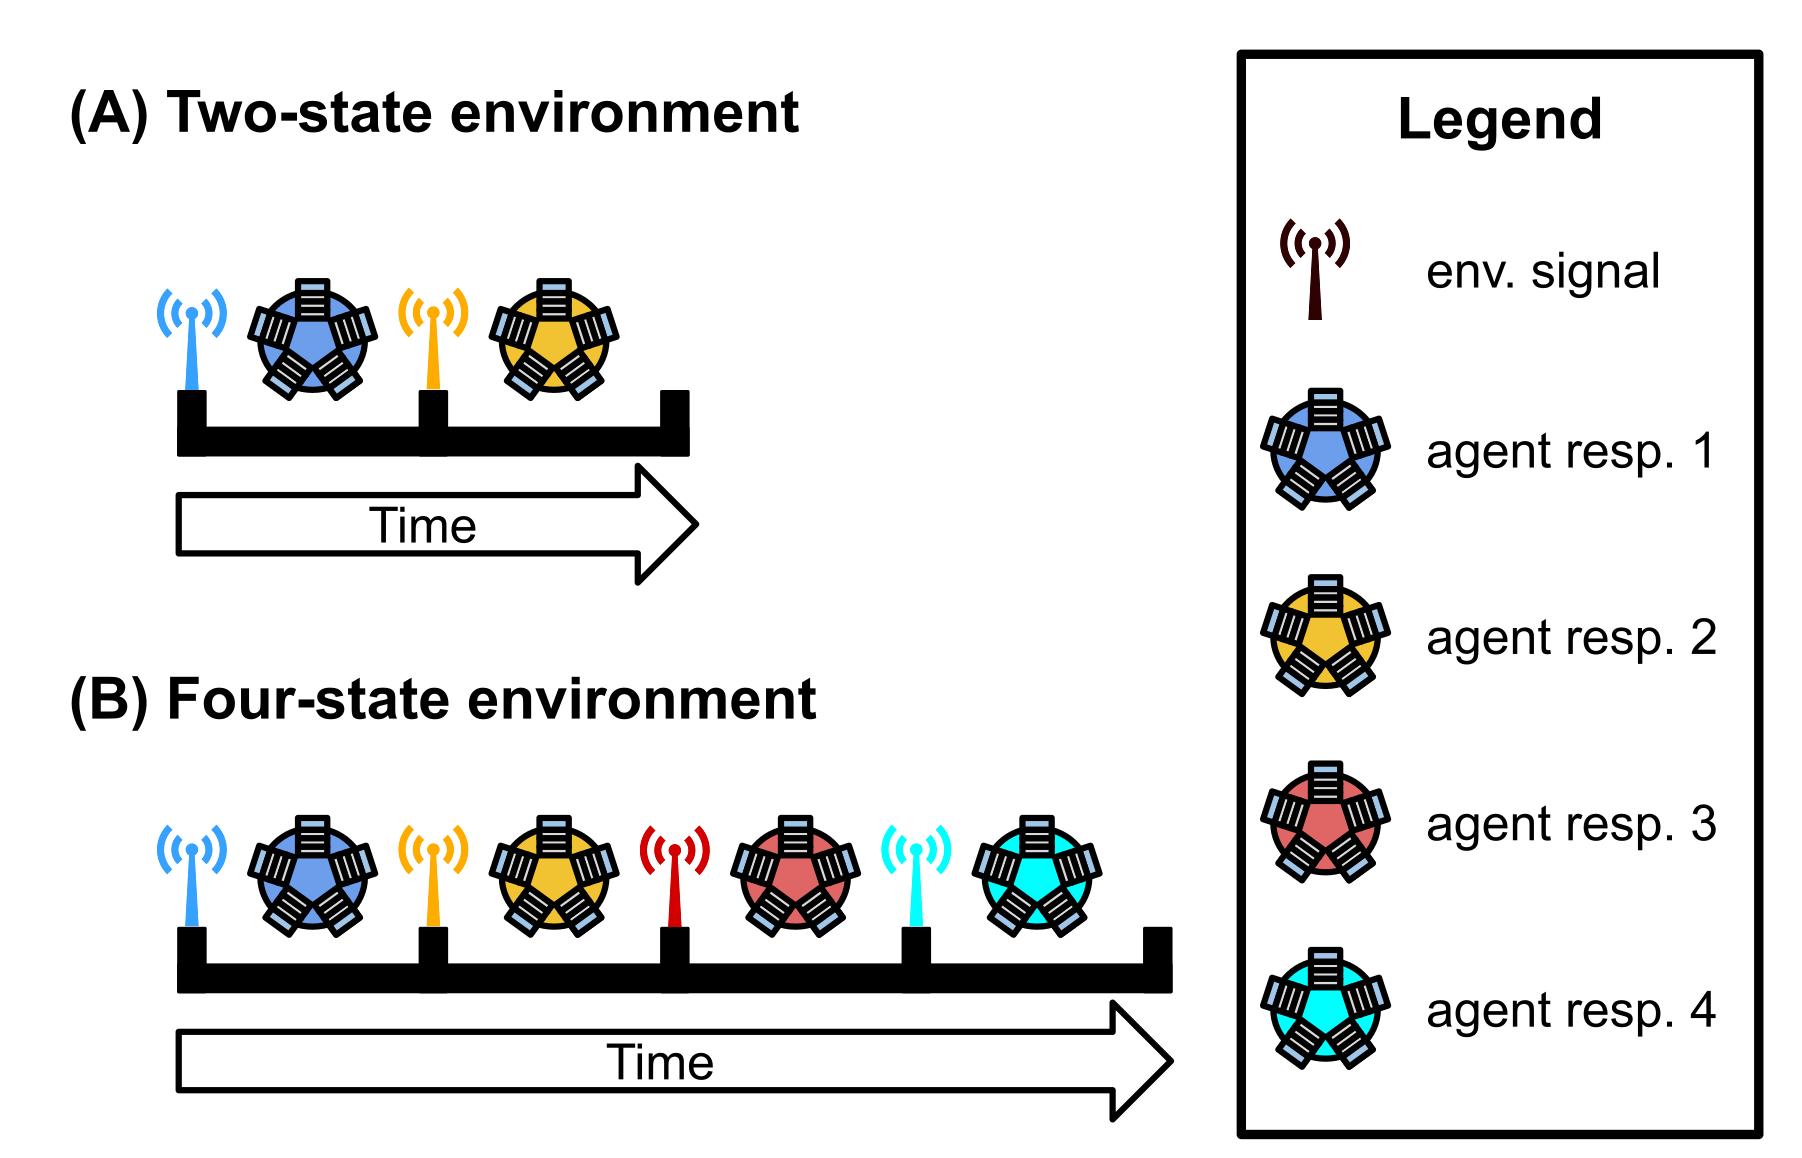
\includegraphics{experiments/2020-11-11-chg-sig/analysis/../../../media/changing-signal-task.png}

Requiring programs to express a distinct instruction in response to each environmental signal represents programs having to perform distinct behaviors.

We afforded programs 128 time steps to express the appropriate response after receiving an environmental signal.
Once the allotted time to respond expires or the program expresses any response, the program's threads of execution are reset, resulting in a loss of all thread-local memory.
\emph{Only} the contents of a program's global memory and each function's regulatory state persist.
The environment then produces the next signal (distinct from all previous signals) to which the program may respond.
A program's fitness is equal to the number of correct responses expressed during evaluation.

We evolved populations of 1000 SignalGP programs to solve the changing-signal task at \(K=16\) (where \(K\) denotes the number of environmental signals).
We evolved populations for \ensuremath{10^{4}} generations or until an program capable of achieving a perfect score during task evaluation (i.e., able to express the appropriate response to each of the \(K\) signals) evolved.

We ran 200 replicate populations (each with a distinct random number seed) of each of the following experimental conditions:

\begin{enumerate}
\def\labelenumi{\arabic{enumi}.}
\tightlist
\item
  a regulation-enabled treatment where programs have access to genetic regulation.
\item
  a regulation-disabled treatment where programs do not have access to genetic regulation.
\end{enumerate}

Note this task does not require programs to shift their response to particular signals over time, and as such, genetic regulation is unnecessary.
Further, because programs experience environmental inputs in a random order, erroneous genetic regulation can manifest as cryptic variation.
For example, non-adaptive down-regulation of a particular response function may be neutral given one sequence of environmental signals, but may be deleterious in another.
\textbf{We expected regulation-enabled SignalGP to exhibit non-adaptive plasticity, potentially resulting in slower adaptation and non-general solutions.}

\hypertarget{analysis-dependencies}{%
\section{Analysis Dependencies}\label{analysis-dependencies}}

Load all required R libraries.

\begin{Shaded}
\begin{Highlighting}[]
\KeywordTok{library}\NormalTok{(ggplot2)}
\KeywordTok{library}\NormalTok{(tidyverse)}
\KeywordTok{library}\NormalTok{(cowplot)}
\KeywordTok{library}\NormalTok{(viridis)}
\KeywordTok{source}\NormalTok{(}\StringTok{"https://gist.githubusercontent.com/benmarwick/2a1bb0133ff568cbe28d/raw/fb53bd97121f7f9ce947837ef1a4c65a73bffb3f/geom\_flat\_violin.R"}\NormalTok{)}
\end{Highlighting}
\end{Shaded}

These analyses were conducted in the following computing environment:

\begin{Shaded}
\begin{Highlighting}[]
\KeywordTok{print}\NormalTok{(version)}
\end{Highlighting}
\end{Shaded}

\begin{verbatim}
##                _                           
## platform       x86_64-pc-linux-gnu         
## arch           x86_64                      
## os             linux-gnu                   
## system         x86_64, linux-gnu           
## status                                     
## major          4                           
## minor          0.2                         
## year           2020                        
## month          06                          
## day            22                          
## svn rev        78730                       
## language       R                           
## version.string R version 4.0.2 (2020-06-22)
## nickname       Taking Off Again
\end{verbatim}

\hypertarget{setup}{%
\section{Setup}\label{setup}}

Load data, initial data cleanup, configure some global settings.

\begin{Shaded}
\begin{Highlighting}[]
\CommentTok{\# Load data file}
\NormalTok{data\_loc \textless{}{-}}\StringTok{ }\KeywordTok{paste0}\NormalTok{(working\_directory, }\StringTok{"data/max\_fit\_orgs.csv"}\NormalTok{)}
\NormalTok{data \textless{}{-}}\StringTok{ }\KeywordTok{read.csv}\NormalTok{(data\_loc, }\DataTypeTok{na.strings=}\StringTok{"NONE"}\NormalTok{)}

\CommentTok{\# Define function to summarize regulation/memory configurations.}
\NormalTok{get\_con \textless{}{-}}\StringTok{ }\ControlFlowTok{function}\NormalTok{(reg, mem) \{}
  \ControlFlowTok{if}\NormalTok{ (reg }\OperatorTok{==}\StringTok{ "0"} \OperatorTok{\&\&}\StringTok{ }\NormalTok{mem }\OperatorTok{==}\StringTok{ "0"}\NormalTok{) \{}
    \KeywordTok{return}\NormalTok{(}\StringTok{"none"}\NormalTok{)}
\NormalTok{  \} }\ControlFlowTok{else} \ControlFlowTok{if}\NormalTok{ (reg }\OperatorTok{==}\StringTok{ "0"} \OperatorTok{\&\&}\StringTok{ }\NormalTok{mem}\OperatorTok{==}\StringTok{"1"}\NormalTok{) \{}
    \KeywordTok{return}\NormalTok{(}\StringTok{"memory"}\NormalTok{)}
\NormalTok{  \} }\ControlFlowTok{else} \ControlFlowTok{if}\NormalTok{ (reg}\OperatorTok{==}\StringTok{"1"} \OperatorTok{\&\&}\StringTok{ }\NormalTok{mem}\OperatorTok{==}\StringTok{"0"}\NormalTok{) \{}
    \KeywordTok{return}\NormalTok{(}\StringTok{"regulation"}\NormalTok{)}
\NormalTok{  \} }\ControlFlowTok{else} \ControlFlowTok{if}\NormalTok{ (reg}\OperatorTok{==}\StringTok{"1"} \OperatorTok{\&\&}\StringTok{ }\NormalTok{mem}\OperatorTok{==}\StringTok{"1"}\NormalTok{) \{}
    \KeywordTok{return}\NormalTok{(}\StringTok{"both"}\NormalTok{)}
\NormalTok{  \} }\ControlFlowTok{else}\NormalTok{ \{}
    \KeywordTok{return}\NormalTok{(}\StringTok{"UNKNOWN"}\NormalTok{)}
\NormalTok{  \}}
\NormalTok{\}}

\CommentTok{\# Specify experimental condition for each datum.}
\NormalTok{data}\OperatorTok{$}\NormalTok{condition \textless{}{-}}\StringTok{ }\KeywordTok{mapply}\NormalTok{(}
\NormalTok{  get\_con,}
\NormalTok{  data}\OperatorTok{$}\NormalTok{USE\_FUNC\_REGULATION,}
\NormalTok{  data}\OperatorTok{$}\NormalTok{USE\_GLOBAL\_MEMORY}
\NormalTok{)}

\NormalTok{data}\OperatorTok{$}\NormalTok{condition \textless{}{-}}\StringTok{ }\KeywordTok{factor}\NormalTok{(}
\NormalTok{  data}\OperatorTok{$}\NormalTok{condition,}
  \DataTypeTok{levels=}\KeywordTok{c}\NormalTok{(}\StringTok{"regulation"}\NormalTok{, }\StringTok{"memory"}\NormalTok{, }\StringTok{"none"}\NormalTok{, }\StringTok{"both"}\NormalTok{)}
\NormalTok{)}

\CommentTok{\# For convenience, create a data set with only solutions}
\CommentTok{\# Filter data to include only replicates labeled as solutions}
\NormalTok{sol\_data \textless{}{-}}\StringTok{ }\KeywordTok{filter}\NormalTok{(}
\NormalTok{  data,}
\NormalTok{  solution}\OperatorTok{==}\StringTok{"1"}
\NormalTok{)}

\CommentTok{\# A lookup table for task complexities}
\NormalTok{task\_label\_lu \textless{}{-}}\StringTok{ }\KeywordTok{c}\NormalTok{(}
  \StringTok{"2"}\NormalTok{ =}\StringTok{ "2{-}signal task"}\NormalTok{,}
  \StringTok{"4"}\NormalTok{ =}\StringTok{ "4{-}signal task"}\NormalTok{,}
  \StringTok{"8"}\NormalTok{ =}\StringTok{ "8{-}signal task"}\NormalTok{,}
  \StringTok{"16"}\NormalTok{ =}\StringTok{ "16{-}signal task"}\NormalTok{,}
  \StringTok{"32"}\NormalTok{ =}\StringTok{"32{-}signal task"}
\NormalTok{)}

\CommentTok{\# Configure our default graphing theme}
\KeywordTok{theme\_set}\NormalTok{(}\KeywordTok{theme\_cowplot}\NormalTok{())}
\end{Highlighting}
\end{Shaded}

\hypertarget{does-regulation-hinder-the-evolution-of-successful-genotypes}{%
\section{Does regulation hinder the evolution of successful genotypes?}\label{does-regulation-hinder-the-evolution-of-successful-genotypes}}

Here, we look at the number of solutions evolved under regulation-enabled and regulation-disabled conditions.
A program is categorized as a `solution' if it can correctly respond to each of the \(K\) environmental signals \emph{during evaluation}.

\begin{Shaded}
\begin{Highlighting}[]
\CommentTok{\# Graph the number of solutions evolved in each condition, faceted by environmental complexity}
\KeywordTok{ggplot}\NormalTok{( sol\_data, }\KeywordTok{aes}\NormalTok{(}\DataTypeTok{x=}\NormalTok{condition, }\DataTypeTok{fill=}\NormalTok{condition) ) }\OperatorTok{+}
\StringTok{  }\KeywordTok{geom\_bar}\NormalTok{() }\OperatorTok{+}
\StringTok{  }\KeywordTok{geom\_text}\NormalTok{(}
    \DataTypeTok{stat=}\StringTok{"count"}\NormalTok{,}
    \DataTypeTok{mapping=}\KeywordTok{aes}\NormalTok{(}\DataTypeTok{label=}\NormalTok{..count..),}
    \DataTypeTok{position=}\KeywordTok{position\_dodge}\NormalTok{(}\FloatTok{0.9}\NormalTok{),}
    \DataTypeTok{vjust=}\DecValTok{0}
\NormalTok{  ) }\OperatorTok{+}
\StringTok{  }\KeywordTok{scale\_x\_discrete}\NormalTok{(}
    \DataTypeTok{name=}\StringTok{"Condition"}\NormalTok{,}
    \DataTypeTok{breaks=}\KeywordTok{c}\NormalTok{(}\StringTok{"memory"}\NormalTok{,}\StringTok{"both"}\NormalTok{),}
    \DataTypeTok{labels=}\KeywordTok{c}\NormalTok{(}\StringTok{"Regulation{-}}\CharTok{\textbackslash{}n}\StringTok{disabled"}\NormalTok{,}\StringTok{"Regulation{-}}\CharTok{\textbackslash{}n}\StringTok{enabled"}\NormalTok{)}
\NormalTok{  ) }\OperatorTok{+}
\StringTok{  }\KeywordTok{ylab}\NormalTok{(}\StringTok{"\# successful replciates (/200)"}\NormalTok{) }\OperatorTok{+}
\StringTok{  }\KeywordTok{theme}\NormalTok{(}\DataTypeTok{legend.position =} \StringTok{"none"}\NormalTok{) }\OperatorTok{+}
\StringTok{  }\KeywordTok{ggtitle}\NormalTok{(}\StringTok{"Successful replicates"}\NormalTok{)}
\end{Highlighting}
\end{Shaded}

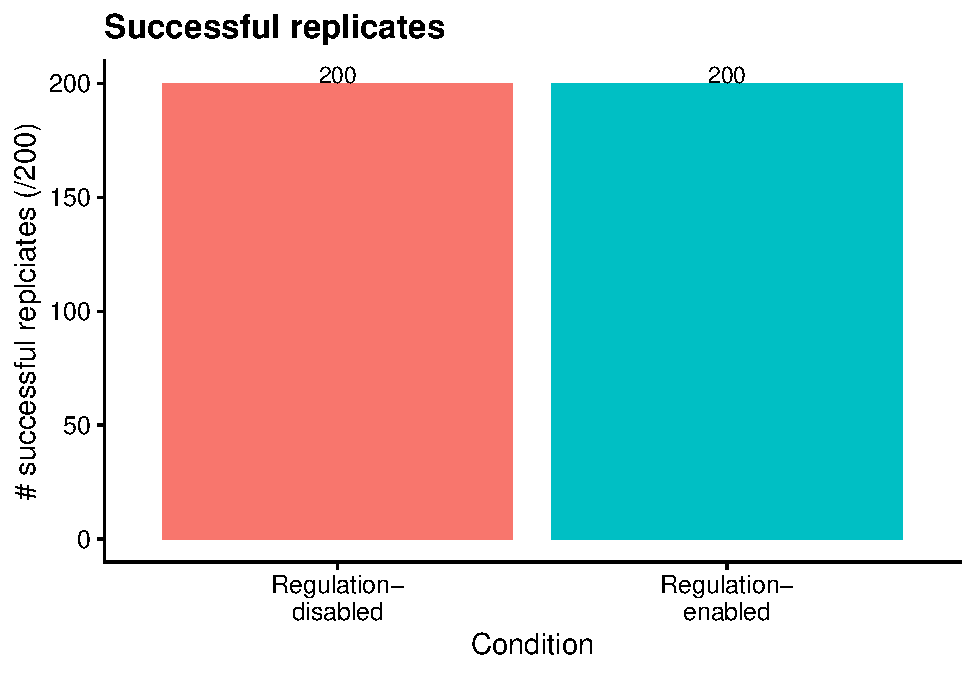
\includegraphics{tag-based-genetic-regulation_files/figure-latex/unnamed-chunk-5-1.pdf}

Programs capable of achieving a perfect score on the changing-signal task (for a given sequence of environment signals) evolve in all 200 replicates of each condition (i.e., with and without access to genetic regulation).
These programs, however, do not necessarily generalize across all possible sequences of environmental signals.

\hypertarget{does-access-to-regulation-slow-adaptation}{%
\subsection{Does access to regulation slow adaptation?}\label{does-access-to-regulation-slow-adaptation}}

I.e., did successful regulation-enabled programs take longer (more generations) to evolve than those evolved in the regulation-disabled treatment?

\begin{Shaded}
\begin{Highlighting}[]
\KeywordTok{ggplot}\NormalTok{( sol\_data, }\KeywordTok{aes}\NormalTok{(}\DataTypeTok{x=}\NormalTok{condition, }\DataTypeTok{y=}\NormalTok{update, }\DataTypeTok{fill=}\NormalTok{condition) ) }\OperatorTok{+}
\StringTok{  }\KeywordTok{geom\_flat\_violin}\NormalTok{(}
    \DataTypeTok{position =} \KeywordTok{position\_nudge}\NormalTok{(}\DataTypeTok{x =} \FloatTok{.2}\NormalTok{, }\DataTypeTok{y =} \DecValTok{0}\NormalTok{),}
    \DataTypeTok{alpha =} \FloatTok{.8}
\NormalTok{  ) }\OperatorTok{+}
\StringTok{  }\KeywordTok{geom\_point}\NormalTok{(}
    \KeywordTok{aes}\NormalTok{(}\DataTypeTok{y =}\NormalTok{ update, }\DataTypeTok{color =}\NormalTok{ condition),}
    \DataTypeTok{position =} \KeywordTok{position\_jitter}\NormalTok{(}\DataTypeTok{width =} \FloatTok{.15}\NormalTok{),}
    \DataTypeTok{size =} \FloatTok{.5}\NormalTok{,}
    \DataTypeTok{alpha =} \FloatTok{0.8}
\NormalTok{  ) }\OperatorTok{+}
\StringTok{  }\KeywordTok{geom\_boxplot}\NormalTok{(}
    \DataTypeTok{width =} \FloatTok{.1}\NormalTok{,}
    \DataTypeTok{outlier.shape =} \OtherTok{NA}\NormalTok{,}
    \DataTypeTok{alpha =} \FloatTok{0.5}
\NormalTok{  ) }\OperatorTok{+}
\StringTok{  }\KeywordTok{scale\_x\_discrete}\NormalTok{(}
    \DataTypeTok{name=}\StringTok{"Condition"}\NormalTok{,}
    \DataTypeTok{breaks=}\KeywordTok{c}\NormalTok{(}\StringTok{"memory"}\NormalTok{, }\StringTok{"both"}\NormalTok{),}
    \DataTypeTok{labels=}\KeywordTok{c}\NormalTok{(}\StringTok{"Regulation{-}}\CharTok{\textbackslash{}n}\StringTok{disabled"}\NormalTok{,}\StringTok{"Regulation{-}}\CharTok{\textbackslash{}n}\StringTok{enabled"}\NormalTok{)}
\NormalTok{  ) }\OperatorTok{+}
\StringTok{  }\KeywordTok{scale\_y\_continuous}\NormalTok{(}
    \DataTypeTok{name=}\StringTok{"Generation first solution evolved }\CharTok{\textbackslash{}n}\StringTok{(log scale)"}\NormalTok{,}
\NormalTok{  ) }\OperatorTok{+}
\StringTok{  }\KeywordTok{guides}\NormalTok{(}\DataTypeTok{fill =} \OtherTok{FALSE}\NormalTok{) }\OperatorTok{+}
\StringTok{  }\KeywordTok{guides}\NormalTok{(}\DataTypeTok{color =} \OtherTok{FALSE}\NormalTok{)}
\end{Highlighting}
\end{Shaded}

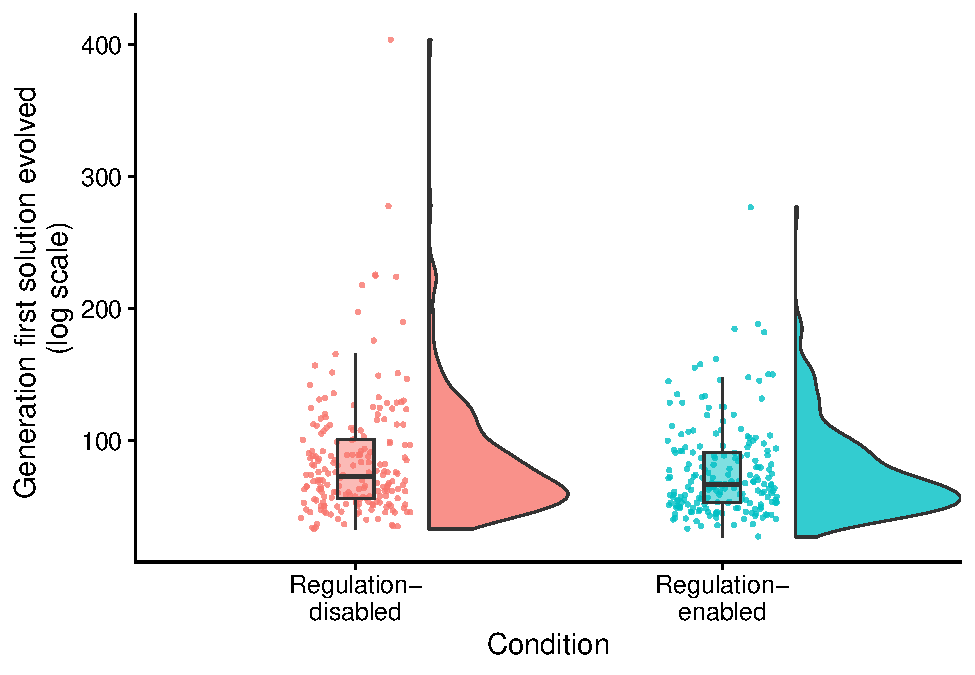
\includegraphics{tag-based-genetic-regulation_files/figure-latex/unnamed-chunk-6-1.pdf}

\begin{Shaded}
\begin{Highlighting}[]
\KeywordTok{print}\NormalTok{(}\KeywordTok{wilcox.test}\NormalTok{(}\DataTypeTok{formula=}\NormalTok{update}\OperatorTok{\textasciitilde{}}\NormalTok{condition, }\DataTypeTok{data=}\NormalTok{data, }\DataTypeTok{exact=}\OtherTok{FALSE}\NormalTok{, }\DataTypeTok{conf.int=}\OtherTok{TRUE}\NormalTok{))}
\end{Highlighting}
\end{Shaded}

\begin{verbatim}
## 
##  Wilcoxon rank sum test with continuity correction
## 
## data:  update by condition
## W = 22188, p-value = 0.05845
## alternative hypothesis: true location shift is not equal to 0
## 95 percent confidence interval:
##  -3.860236e-05  1.000000e+01
## sample estimates:
## difference in location 
##               5.000013
\end{verbatim}

The difference in the number of generations before a solution arises is not significantly different.

\hypertarget{do-they-generalize}{%
\subsection{Do they generalize?}\label{do-they-generalize}}

Note that solutions may or may not generalize beyond the sequence of environmental signals on which they achieved a perfect score (and were thus categorized as a `solution').
We re-evaluated each `solution' on a random sample of 5000 sequences of environmental signals to test for generalization.
We deem programs as having successfully generalized only if they responded correctly in all 5000 tests.

To see if regulation is preventing some regulation-enabled solutions from generalizing, we test generalization for regulation-enabled solutions with their regulation faculties knocked out (i.e., regulation instructions replaced with no-operations).

\begin{Shaded}
\begin{Highlighting}[]
\CommentTok{\# Grab count data to make bar plot life easier}
\NormalTok{num\_solutions\_reg \textless{}{-}}\StringTok{ }\KeywordTok{length}\NormalTok{(}\KeywordTok{filter}\NormalTok{(data, condition}\OperatorTok{==}\StringTok{"both"} \OperatorTok{\&}\StringTok{ }\NormalTok{solution}\OperatorTok{==}\StringTok{"1"}\NormalTok{)}\OperatorTok{$}\NormalTok{SEED)}
\NormalTok{num\_generalize\_reg \textless{}{-}}\StringTok{ }\KeywordTok{length}\NormalTok{(}\KeywordTok{filter}\NormalTok{(data, condition}\OperatorTok{==}\StringTok{"both"} \OperatorTok{\&}\StringTok{ }\NormalTok{all\_solution}\OperatorTok{==}\StringTok{"1"}\NormalTok{)}\OperatorTok{$}\NormalTok{SEED)}
\NormalTok{num\_generalize\_ko\_reg \textless{}{-}}\StringTok{ }\KeywordTok{length}\NormalTok{(}\KeywordTok{filter}\NormalTok{(data, condition}\OperatorTok{==}\StringTok{"both"} \OperatorTok{\&}\StringTok{ }\NormalTok{all\_solution\_ko\_reg}\OperatorTok{==}\StringTok{"1"}\NormalTok{)}\OperatorTok{$}\NormalTok{SEED)}

\NormalTok{num\_generalize\_mem \textless{}{-}}\StringTok{ }\KeywordTok{length}\NormalTok{(}\KeywordTok{filter}\NormalTok{(data, condition}\OperatorTok{==}\StringTok{"memory"} \OperatorTok{\&}\StringTok{ }\NormalTok{all\_solution}\OperatorTok{==}\StringTok{"1"}\NormalTok{)}\OperatorTok{$}\NormalTok{SEED)}

\NormalTok{sol\_cnts \textless{}{-}}\StringTok{ }\KeywordTok{data.frame}\NormalTok{(}\DataTypeTok{x=}\DecValTok{1}\OperatorTok{:}\DecValTok{3}\NormalTok{)}
\NormalTok{sol\_cnts}\OperatorTok{$}\NormalTok{type \textless{}{-}}\StringTok{ }\KeywordTok{c}\NormalTok{(}\StringTok{"reg\_generalize"}\NormalTok{, }\StringTok{"reg\_generalize\_ko\_reg"}\NormalTok{, }\StringTok{"mem\_generalize"}\NormalTok{)}
\NormalTok{sol\_cnts}\OperatorTok{$}\NormalTok{val \textless{}{-}}\StringTok{ }\KeywordTok{c}\NormalTok{(num\_generalize\_reg, num\_generalize\_ko\_reg, num\_generalize\_mem)}

\KeywordTok{ggplot}\NormalTok{( sol\_cnts, }\KeywordTok{aes}\NormalTok{(}\DataTypeTok{x=}\NormalTok{type, }\DataTypeTok{y=}\NormalTok{val, }\DataTypeTok{fill=}\NormalTok{type) ) }\OperatorTok{+}
\StringTok{  }\KeywordTok{geom\_bar}\NormalTok{(}\DataTypeTok{stat=}\StringTok{"identity"}\NormalTok{) }\OperatorTok{+}
\StringTok{  }\KeywordTok{geom\_text}\NormalTok{(}
    \KeywordTok{aes}\NormalTok{(}\DataTypeTok{label=}\NormalTok{val),}
    \DataTypeTok{stat=}\StringTok{"identity"}\NormalTok{,}
    \DataTypeTok{position=}\KeywordTok{position\_dodge}\NormalTok{(}\FloatTok{0.75}\NormalTok{),}
    \DataTypeTok{vjust=}\OperatorTok{{-}}\FloatTok{0.01}
\NormalTok{  ) }\OperatorTok{+}
\StringTok{  }\KeywordTok{scale\_x\_discrete}\NormalTok{(}
    \DataTypeTok{name=}\StringTok{"Condition"}\NormalTok{,}
    \DataTypeTok{limits=}\KeywordTok{c}\NormalTok{(}
      \StringTok{"mem\_generalize"}\NormalTok{,}
      \StringTok{"reg\_generalize"}\NormalTok{,}
      \StringTok{"reg\_generalize\_ko\_reg"}
\NormalTok{      ),}
    \DataTypeTok{labels=}\KeywordTok{c}\NormalTok{(}
      \StringTok{"Regulation{-}}\CharTok{\textbackslash{}n}\StringTok{disabled"}\NormalTok{,}
      \StringTok{"Regulation{-}}\CharTok{\textbackslash{}n}\StringTok{enabled"}\NormalTok{,}
      \StringTok{"Regulation{-}}\CharTok{\textbackslash{}n}\StringTok{enabled}\CharTok{\textbackslash{}n}\StringTok{(reg. KO)"}
\NormalTok{    )}
\NormalTok{  ) }\OperatorTok{+}
\StringTok{  }\KeywordTok{scale\_y\_continuous}\NormalTok{(}
    \DataTypeTok{name=}\StringTok{"\# of solutions that generalize"}\NormalTok{,}
    \DataTypeTok{limits=}\KeywordTok{c}\NormalTok{(}\DecValTok{0}\NormalTok{, }\DecValTok{210}\NormalTok{),}
    \DataTypeTok{breaks=}\KeywordTok{seq}\NormalTok{(}\DecValTok{0}\NormalTok{,}\DecValTok{200}\NormalTok{,}\DecValTok{50}\NormalTok{)}
\NormalTok{  ) }\OperatorTok{+}
\StringTok{  }\KeywordTok{theme}\NormalTok{(}
    \DataTypeTok{legend.position=}\StringTok{"none"}\NormalTok{,}
    \DataTypeTok{axis.text.x =} \KeywordTok{element\_text}\NormalTok{(}\DataTypeTok{size=}\DecValTok{10}\NormalTok{)}
\NormalTok{  ) }\OperatorTok{+}
\StringTok{  }\KeywordTok{ggsave}\NormalTok{(}\KeywordTok{paste0}\NormalTok{(working\_directory, }\StringTok{"imgs/chg{-}env{-}16{-}generalization.png"}\NormalTok{), }\DataTypeTok{width=}\DecValTok{4}\NormalTok{,}\DataTypeTok{height=}\DecValTok{4}\NormalTok{)}
\end{Highlighting}
\end{Shaded}

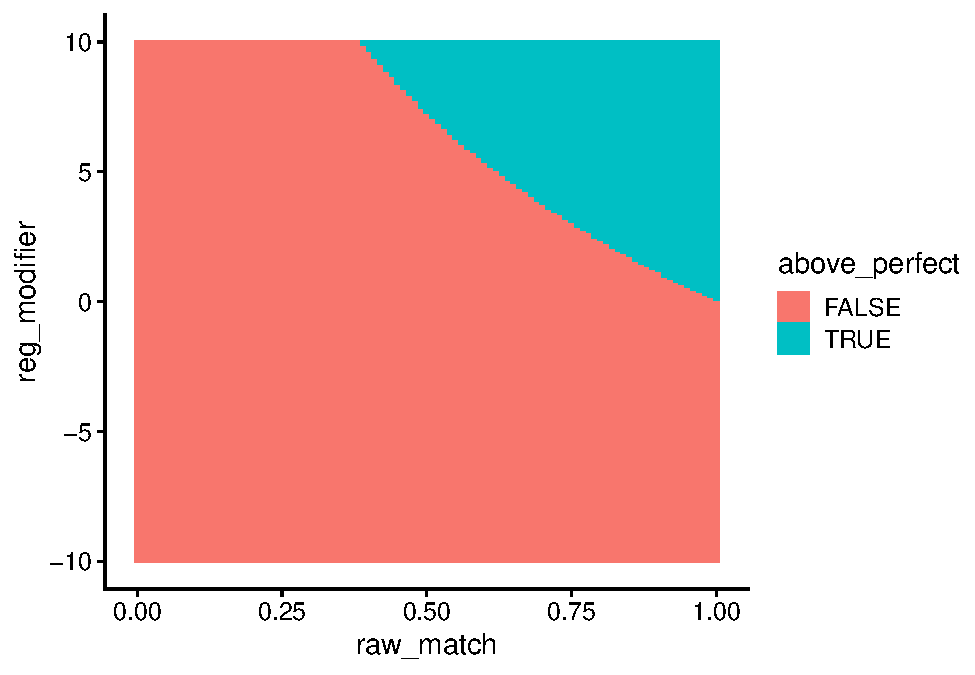
\includegraphics{tag-based-genetic-regulation_files/figure-latex/unnamed-chunk-7-1.pdf}

All regulation-disabled programs successfully generalized.

\begin{Shaded}
\begin{Highlighting}[]
\NormalTok{table \textless{}{-}}\StringTok{ }\KeywordTok{matrix}\NormalTok{(}\KeywordTok{c}\NormalTok{(num\_generalize\_reg,}
\NormalTok{                  num\_generalize\_mem,}
                  \DecValTok{200} \OperatorTok{{-}}\StringTok{ }\NormalTok{num\_generalize\_reg,}
                  \DecValTok{200} \OperatorTok{{-}}\StringTok{ }\NormalTok{num\_generalize\_mem),}
                \DataTypeTok{nrow=}\DecValTok{2}\NormalTok{)}
\KeywordTok{rownames}\NormalTok{(table) \textless{}{-}}\StringTok{ }\KeywordTok{c}\NormalTok{(}\StringTok{"reg{-}augmented"}\NormalTok{, }\StringTok{"reg{-}disabled"}\NormalTok{)}
\KeywordTok{colnames}\NormalTok{(table) \textless{}{-}}\StringTok{ }\KeywordTok{c}\NormalTok{(}\StringTok{"success"}\NormalTok{, }\StringTok{"fail"}\NormalTok{)}
\KeywordTok{fisher.test}\NormalTok{(table)}
\end{Highlighting}
\end{Shaded}

\begin{verbatim}
## 
##  Fisher's Exact Test for Count Data
## 
## data:  table
## p-value = 5.113e-06
## alternative hypothesis: true odds ratio is not equal to 1
## 95 percent confidence interval:
##  0.0000000 0.2115509
## sample estimates:
## odds ratio 
##          0
\end{verbatim}

The difference in number of generalizing solutions between regulation-enabled and regulation-disabled conditions is statistically significant (Fisher's exact test).

Moreover, 5 of the 18 non-generalizing programs generalize when we knockout genetic regulation.
Upon close inspection, the other 13 non-general programs relied on genetic regulation to achieve initial success but failed to generalize to arbitrary environment signal sequences.

\end{document}
